\documentclass[a4paper]{exam}
\usepackage[english]{babel}
\usepackage[fleqn]{amsmath}
\usepackage{amsthm}
\usepackage{amssymb}
\usepackage{amsmath}
\usepackage{mathtools}
\usepackage{enumerate}
\usepackage{tabstackengine}
\usepackage{thmtools}
\usepackage{xcolor}
\usepackage{bookmark}
\usepackage{pdfpages}
% start maubach toegevoegd
\usepackage{hyperref} % deze regel is veranderd, stond hierboven
\usepackage{makeidx} % deze regel is toegevoegd.
\usepackage[makeroom]{cancel} % deze regel is toegevoegd.
\newtheorem*{voorbeeld}{Voorbeeld}
% einde maubach toegevoegd

\makeatletter
\renewcommand\@seccntformat[1]{}
\makeatother

\theoremstyle{definition}
\newtheorem*{define}{Definitie}
\newtheorem*{theorem}{Stelling}
\newtheorem*{lemma}{Lemma}
\newtheorem*{opm}{Opmerking}
\newtheorem*{gevolg}{Gevolg}
\newtheorem*{nota}{Notatie}
\newtheorem*{valkuil}{\textcolor{red}{Valkuil}}
\newtheorem*{note}{\textcolor{red}{Note}}

%\DeclareMathOperator{\intr}{int}
%\DeclareMathOperator{\dist}{dist}
\DeclareMathOperator{\intr}{\mathop{int}}
\DeclareMathOperator{\dist}{\mathop{dist}}

%--------------------Make usable space all of page
\setlength{\oddsidemargin}{0in}
\setlength{\evensidemargin}{0in}
\setlength{\topmargin}{0in}
\setlength{\headsep}{-.25in}
\setlength{\textwidth}{6.5in}
\setlength{\textheight}{8.5in}

%--------------------Indention
\newlength\tindent
\setlength{\tindent}{\parindent}
\setlength{\parindent}{0pt}
\renewcommand{\indent}{\hspace*{\tindent}}

\stackMath
\makeatletter\renewcommand\TAB@delim[1]{\displaystyle#1}\makeatother
\setstackEOL{\cr}% ROW DELIMITER FOR STACKS
\renewcommand\stackalignment{l}% LEFT ALIGNMENT OF STACKS
\setstackgap{S}{8pt}% INTER-ROW PADDING OF SHORT STACKS

% Number sets
\newcommand{\naturals}{\mathbb{N}}
\newcommand{\reals}{\mathbb{R}}
\newcommand{\complex}{\mathbb{C}}
\newcommand{\rationals}{\mathbb{Q}}
%start nieuwe macros
\def\set#1{\lbrace#1\rbrace}
\def\abs#1{{\left|#1\right|}}
\def\vectorstat#1{{\textbf{#1}}}
\protected\def\a{\vectorstat{a}}
\protected\def\b{\vectorstat{b}}
\protected\def\c{\vectorstat{c}}
\protected\def\d{\vectorstat{d}}
\protected\def\e{\vectorstat{e}}
\protected\def\f{\vectorstat{f}}
\protected\def\g{\vectorstat{g}}
\protected\def\h{\vectorstat{h}}
%\protected\def\i{\vectorstat{i}}
\protected\def\j{\vectorstat{j}}
\protected\def\k{\vectorstat{k}}
\protected\def\l{\vectorstat{l}}
\protected\def\m{\vectorstat{m}}
\protected\def\n{\vectorstat{n}}
\protected\def\p{\vectorstat{p}}
\protected\def\q{\vectorstat{q}}
\protected\def\r{\vectorstat{r}}
\protected\def\s{\vectorstat{s}}
\protected\def\t{\vectorstat{t}}
\protected\def\u{\vectorstat{u}}
\protected\def\v{\vectorstat{v}}
\protected\def\w{\vectorstat{w}}
\protected\def\x{\vectorstat{x}}
\protected\def\y{\vectorstat{y}}
\protected\def\z{\vectorstat{z}}
\protected\def\A{\vectorstat{A}}
\protected\def\B{\vectorstat{B}}
\protected\def\C{\vectorstat{C}}
\protected\def\D{\vectorstat{D}}
\protected\def\E{\vectorstat{E}}
\protected\def\F{\vectorstat{F}}
\protected\def\G{\vectorstat{G}}
\protected\def\H{\vectorstat{H}}
\protected\def\I{\vectorstat{I}}
\protected\def\J{\vectorstat{J}}
\protected\def\K{\vectorstat{K}}
\protected\def\L{\vectorstat{L}}
\protected\def\M{\vectorstat{M}}
\protected\def\N{\vectorstat{N}}
\protected\def\P{\vectorstat{P}}
\protected\def\Q{\vectorstat{Q}}
\protected\def\R{\vectorstat{R}}
\protected\def\S{\vectorstat{S}}
\protected\def\T{\vectorstat{T}}
\protected\def\U{\vectorstat{U}}
\protected\def\V{\vectorstat{V}}
\protected\def\W{\vectorstat{W}}
\protected\def\X{\vectorstat{X}}
\protected\def\Y{\vectorstat{Y}}
\protected\def\Z{\vectorstat{Z}}
\protected\def\zero{\vectorstat{0}}
\protected\def\one{\vectorstat{1}}
\protected\def\two{\vectorstat{2}}
\def\up#1{^{(#1)}}
\protected\def\red#1{{\color{red}#1}}
\protected\def\ore#1{{\color{orange}#1}}
\protected\def\grn#1{{\color{green}#1}}
\protected\def\blu#1{{\color{blue}#1}}
\protected\def\brn#1{{\color{brown}#1}}
\protected\def\blk#1{{\color{black}#1}}
\protected\def\gry#1{{\color{gray}#1}}
\protected\def\mgn#1{{\color{magenta}#1}}
\protected\def\prp#1{{\color{purple}#1}}
\newcommand{\indx}[1]{\index{#1}{\sl #1}}%
\def\exclamation{!}% use \exclamation instead of '!' inside \indx ('!' is active in \index)
\makeindex%
%einde nieuwe macros


\begin{document}
	\section{Beste allemaal}
	
	Mijn complimenten -- dit is de eerste keer dat ``m'n'' studenten alle lecture notes in \LaTeX typen.
	Prima job!
	
	\ \\
	Ik heb leesbare tekst toegevoegd (in \blu{blauw}).
	
	\ \\
	Ik heb in het \verb$.tex$ bestand definities toegevoegd -- geen aktie noodzakelijk -- tussen
	``start nieuwe macros'' en ``einde nieuwe macros'' die het
	typewerk sterk kunnen vergemakkelijken. ``Makkelijk'' is smaakafhankelijk.
	
	\ \\
	Ik stel voor -- maar dat hoeft vanzelfsprekend niet -- dat ``jullie'' de typografie aanpassen aan wat in de Analyse/Calculus gebruikelijk is -- een deel heb ik al als voorbeeld voorgedaan in de brontekst van dit bestand:
	\begin{itemize}
		\item In plaats van de letter x, y en z \textbf{die vectoren zijn in dit} \verb$.tex$ \textbf{bestand}, type
		\verb$\x$, \verb$\y$ en \verb$\z$: $\x, \y, \z$
		\item Voor alle vectoren zoals $\mathbf{a}$, $\mathbf{b}$ etc: Type \verb$\a$, \verb$\b$, etc
		\item Ditto voor vectorwaardige functies \verb$\f\colon\reals^d\mapsto\reals$: $\f\colon\reals^d\mapsto\reals$: Type \verb$\f$
		\item In plaats van de letter 0 type voor nulvectoren \verb$\zero$: $\zero$
		\item In plaats van \verb$|x|$ type \verb$\abs{x}$: $\abs{x}$
		\item In plaats van \verb$|\x|$ type \verb$\abs{\x}$: $\abs{\x}$
		\item In plaats van \verb$x^{(n)}$ type \verb$x\up{n}$: $x\up{n}$
		\item In plaats van \verb$\x^{(n)}$ type \verb$\x\up{n}$: $\x\up{n}$
		\item In plaats van \verb$\Leftrightarrow$ type \verb$\iff$: $\iff$
		\item In plaats van \verb$\Rightarrow$ type \verb$\implies$: $\implies$
		\item In plaats van \verb$\mathbb{R}$ type \verb$\reals$: $\reals$ (heb ik al vervangen)
		\item In plaats van \verb$\mathbb{N}$ type \verb$\naturals$: $\naturals$ (heb ik al vervangen)
		\item In plaats van \verb$:$ type \verb$\colon$: $x\colon y$
		\item Voor verzamelingen type bv \verb$\set{1,2,3}$: $\set{1,2,3}$
		\item Voor rode tekst gebruik \verb$\red{word 1 and 2}$ type \verb$\red{word 1 and 2}$: \red{word 1 and 2}
		\item Voor groene tekst gebruik \verb$\grn{word 1 and 2}$ type \verb$\grn{word 1 and 2}$: \grn{word 1 and 2}
		\item Voor blauwe tekst gebruik \verb$\blu{word 1 and 2}$ type \verb$\blu{word 1 and 2}$: \blu{word 1 and 2}
		\item \blu{Het} \verb$\blu{...}$ \blu{kleuren commando kan geen} \verb#\verb$...$# \blu{constructie bevatten.}
		\item De langere variant \verb$\{\color{blue}...}$ kan wel \verb#\verb$...$# in de \dots bevatten!
		\item De langere variant \verb$\{\color{red}...}$ kan wel \verb#\verb$...$# in de \dots bevatten!
		\item De langere variant \verb$\{\color{green}...}$ kan wel \verb#\verb$...$# in de \dots bevatten!
		\item In plaats van \verb$\define$ type \verb$\begin{define}[onderwerp] ..... \end{define}$: zie voorbeelden in dit \verb$.tex$ bestand
		\item Om een \verb$woord$ in de index te plaatsen, type \verb$\indx{woord}$ -- het verschijnt dan ``slanted'' in de \verb$.pdf$
		\item In \LaTeX\ zijn de braces \verb${...}$ de \LaTeX\ groep-open en \LaTeX\ groep-sluit operatoren -- en daarom niet zichtbaar in de tekst. Om ze zichtbaar te maken moet je \verb$\lbrace$ resp.{} \verb$\rbrace$ typen of -- minder slim als je \LaTeX\ beter kent type je \verb$\{$ resp.{} \verb$\}$.
		\item Als je zulke braces (\verb$\{\}$, \verb$()$, \verb$[]$) groot genoeg wilt hebben dan type je \verb$\left\lbrace ... \right\rbrace$:
		\[
		\left\lbrace \int_0^1 f(x) \text{d}x \right\rbrace.
		\]
		Een minder alternatief -- alleen te snappen met meer \LaTeX\ kennis is \verb$\big\{$ ipv.{} \verb$\left\rbrace$.
		\item Als je in het \verb$.pdf$ wilt kunnen klikken op secties om daarnaar toe te springen includeer dan
		\verb$\usepackage{hyperref}$ -- heb ik al gedaan -- dit package was al wel geincludeerd maar het automatisch springen was uitgeschakeld.
		\item De definities van \verb$\intr$ en \verb$\distr$ heb ik aangepast -- dat valt niet op maar daar komt later voordeel van
		\item De \verb$\AA$ geeft niet de gewenst ``interior'' notatie -- daarom heb ik \verb$\AA$ aangepast aan de \LaTeX\ standaard
		om $\mathring{A}$ te geven
		\item In plaats van \verb$\lim_{n\rightarrow\infty}$ type de kortere \LaTeX\ standaard \verb$\lim_{n\to\infty}$: $\lim_{n\to\infty}$
		\item De bold -- vetgedrukte -- vectoren veranderen in underline vectoren door 1 regel te wijzigen!
		\item In math mode -- tussen dollars en \verb$\[\]$ gebruik \verb$\ldots$ voor enumeraties zoals \verb$1,2,\ldots,d$: $1,2,\ldots,d$ -- gebruik \verb$\dots$ alleen in text mode.
	\end{itemize}
	Ik stel voor dat jullie deze tips verhuizen naar de appendix voor de volgende generatie -- die appendix heb ik toegevoegd.
	
	\ \\
	Groet,
	
	Jos.
	
	\newpage
	\section{Inleiding}
	We nemen aan dat $d\in\naturals_+$.
	
	\section{College 15}
	\subsection{Eigenschappen van de norm}
	\blu{Voor alle $\x\in \reals^d$ en $c\in\reals$ moet gelden}
	\begin{enumerate}[(i)]
		\item $|\x| \geq 0$
		\item \blu{$\abs{\x}=0 \Leftrightarrow \x=\zero$}
		\item $|c\x|=|c||\x|$ ($|$norm$|$ = $|$absolute waarde$||$norm$|$)
	\end{enumerate}
	\blu{Als} \verb#|.|# \blu{een norm is dan geldt voor alle $\x,\y\in \reals^d$ de:}
	\begin{enumerate}[(i)]
		\item ongelijkheid van \indx{Cauchy-Schwartz}
		\[\forall \x,\y \in \reals^d: \sum_{i=1}^{d}\x_i \y_i = (\x,\y)\]
		\[|(\x,\y)| \leq |\x||\y|\]
		\item \indx{driehoeksongelijkheid}
		\[\forall \x,\y \in \reals^d: |\x+\y|\leq |\x|+|\y|\]
	\end{enumerate}
	\subsection{Afstand in $\reals^d$}
	\begin{define}
		\blu{Een afstands functie $(\x,\y)\mapsto\dist(\x,\y)\in\reals$ heeft de eigenschap dat voor alle $\x,\y\in\reals^d$:}
		\begin{align*}
		\blu{\dist(\x,\y)} & \geq 0 \\
		\blu{\dist(\x,\y)} & =0 \Leftrightarrow \x=\y \\
		\blu{\dist(\x,\y)} & \leq \blu{\dist(\x,\z) + \dist(\z,\y)}
		\end{align*}
	\end{define}
	\blu{De meest gebruikte afstandsfunctie in $\reals^d$ is $\dist(\x,\y):=|\x-\y|$}
	
	\begin{define}[Bol]
		Laat $\x\in\reals^d$ en laat \blu{$0<\blu{r}\in\reals$}. Dan is \blu{de \indx{bol}\ om $\x$ met straal $r$ de verzameling}
		\[
		B(x,r)=\set{y \in \reals^d \blu{\colon} \abs{y-x}<r}.
		\]
		\cancel{rond $x$ met straal $r$.}
	\end{define}
	\begin{define}[Inwendig punt] Zij $\x \in \reals^d$ and $A \subset \reals^d$. Dan is $\x$ een
		\indx{inwendig punt}/(\textit{interior point}) van $A$
		als er $\exists_{r>0}\colon B(\x,r) \subset A$.
		\blu{In dat geval heten $A$ en $\B(\x,r)$} een \indx{omgeving}/(\textit{neighbourhood}) van $\x$.
	\end{define}
	\begin{define}[Inwendige $\mathring{A}$, open \blu{verzameling} $A$]
		Het inwendige van $A$ is
		\[\intr A=\mathring{A}=\left\lbrace x \in A \colon \x \text{ inwendig punt van } A\right\rbrace\]
		$A$ heet \indx{open verzameling}\ als $A=\mathring{A}$ oftewel als
		\[
		\forall _{x \in A} \exists _{R \in (0,\infty)}\colon B(x,R) \subset A,
		\]
		oftewel elk punt van $A$ is een inwendig punt.
	\end{define}
	\begin{theorem}
		\begin{enumerate}[(1)]
			\item Zij $\left\lbrace A_\alpha \bigm| \alpha \in I \right\rbrace$ een familie van open verzamelingen $A_\alpha \subset \reals^d$. Dan \blu{is}
			\[
			\bigcup_{\alpha \in I}A_\alpha
			\]
			open.
			\item Zij $A_1,A_2,\dots,A_n \in \reals^d$ open. Dan \blu{is}
			\[
			\bigcap_{i=1}^{n}A_i
			\]
			open.
		\end{enumerate}
	\end{theorem}
	\begin{theorem}[Open]
		\blu{Zij $A\in\reals^d$. Dan is}
		\item \[\intr A=\bigcup_{C \subset A, C \text{ open} }C=\bigcup \left\lbrace C \colon C \subset A \blu{\wedge} C \text{ is open}\right\rbrace\]
		open. Volgt uit \cancel{(i) en} \blu{Kosmala} 10.1.4
	\end{theorem}
	\begin{define}[Rand]
		\blu{Zij $A \subset \reals^d$.} Dan
		\[\partial A:= \reals^d\backslash (\intr A \cup \intr (\reals^d\backslash A))\]
		d.w.z: $x$ is een randpunt van $A \iff x$ is geen inwendig punt van $A$ en geen inwendig punt van het complement $\reals^d\backslash A$.
		\blu{Equivalente definitie: Als $\x$ een randpunt is dan geldt voor alle $0<r\in\reals$ dat
			$B(\x,r)$ zowel een punt van $A$ als van $\reals\backslash A$ bevat.}
	\end{define}
	\begin{lemma}
		\blu{Zij $A\in\reals^d$.}
		Elke $x \in \reals$ hoort precies \blu{in} 1 \blu{(exclusive or)} van de drie verzamelingen
		\begin{enumerate}
			\item $\intr A$
			\item $\intr (\reals^d\backslash A)$
			\item $\partial A$.
		\end{enumerate}
	\end{lemma}
	\blu{\begin{voorbeeld}
			Zij $A = [0,1]$ dan is $\intr A=(0,1)$, $\intr (\reals^d\backslash A)=(-\infty,0)\cup(1,\infty)$
			and $\partial A = \set{0,1}$.
		\end{voorbeeld}
	}
	\subsection{Stellingen uit het huiswerk}
	\begin{theorem}
		$\x \in \reals^d$, $0<r\in\reals$, dan \blu{is} $B(\x,r)$ open.
	\end{theorem}
	\newpage
	\section{College 16}
	\subsection{Convergentie in $\reals^d$}
	\begin{define}
		Zij \blu{$(\x\up{n}) = (x\up{1}_1,x\up{1}_2,\ldots,x\up{1}_d), (x\up{2}_1,x\up{2}_2,\ldots,x\up{2}_d), \ldots$}
		%\cancel{$(\underline{x}^{(n)}) = ((x^{(1)},\dots ,x^{(1)}),(x^{(2)},\dots ,x^{(2)}),\dots )$}
		een rij in $\reals^d$\cancel{,} en $\blu{\a} =(a_1, \dots ,a_d ) \in \reals^d$. \blu{Dan heet} $(\x^{(n)})$ convergent naar $\a$ als
		\begin{enumerate}[(i)]
			\item $\abs{\x\up{n}-\a}\stackrel{n\rightarrow \infty}{\longrightarrow} 0$
			\item $\forall _{\varepsilon >0} \exists _{n_0=n_0(\varepsilon)}: \forall _{n\geq n_0} : \abs{\x\up{n} - a} < \varepsilon$.
			\item $\forall _{\varepsilon >0} \exists _{n_0=n_0(\varepsilon)}: \forall _{n\geq n_0} : \x\up{n} \in B(\a,\varepsilon )$
		\end{enumerate}
	\end{define}		
	\begin{theorem}
		$\lim_{n\rightarrow\infty}\x\up{n}=\a \iff \lim_{n\to\infty} x\up{n}_{i} = a_i$ voor \blu{alle} $i=1,\cancel{\dots}\ldots ,d$.
	\end{theorem}
	
	\define[verdichtingspunt] Zij $A \subset \reals^d$. Een punt $x \in \reals^d$ heet \indx{verdichtingspunt} van $A$ als \[\forall _{R>0}:B(x,R)\cap  A \backslash\{x\} \neq \emptyset.\]
	Dan $A':=\big\{ x \in \reals^d \bigm| x \text{ verdichtingspunt van } A\big\}$ \blu{is de verzameling van
		alle verdichtingspunten van $A$}.
	
	\lemma Zij $A \subset \reals^d$. Dan $\partial A \subset A\cup A'$.
	\define $A \subset \reals^d$ heet \textbf{gesloten} als haar \underline{complement open} is.
	\valkuil Een niet open/gesloten verzameling is in het algemeen niet gesloten/open.
	\blu{Niet alle verzamelingen zijn open en of gesloten. Sommige verzamelingen zoals $[0,1)$ zijn geen van beide
		en sommige andere verzamelingen zoals $\reals$ zijn zowel open als gesloten.}
	
	\theorem[Karakterisering voor geslotenheid] Zij $A \subset \reals^d$. De volgende beweringen zijn equivalent:
	\begin{enumerate}[(i)]
		\item $A$ gesloten
		\item $A'\subset A$
		\item $\partial A \subset A$
		%\item voor elke convergente rij in $A$ ligt de limiet in $A$. (limiet convergente rij blijft in $A$)
		\item voor elke convergente rij \blu{$(\x\up{n})\to\x$ met $\set{\x\up{n}}\subset A$ geldt dat de limiet in $\x\in A$.}% (limiet convergente rij blijft in $A$)
	\end{enumerate}
	
	\theorem $\left[\text{K}\right]$ 10.1.6
	\begin{enumerate}[(i)]
		\item Zij $\big\{ A_\alpha \bigm| \alpha \in I \big\}$ een familie gesloten verzamelingen $A_\alpha \subset \reals^d$. Dan $\bigcap_{\alpha \in I}A_\alpha$ gesloten.
		\item Zij $A_1, \dots ,A_n$ gesloten. Dan $\bigcup_{i=1}^n A_i$ gesloten.
	\end{enumerate}
	
	\define[afsluiting] Zij $A \subset \reals^d$. De verzameling $\overline{A}:= \reals^d \backslash (\intr (\reals^d \backslash A))$ heet de \indx{afsluiting} (\textit{closure}) van $A$.
	\theorem[Karakterisering \cancel{voor} \blu{van} de afsluiting]
	Zij $A \subset \reals^d$. Dan
	\[\overline{A}= A \cup \partial A = A \cup A'= \big\{\z \in \reals^d \bigm| \exists _{\text{rij } (\x\up{n}) \text{ in } A \text{ met } \x\up{n} \to \z} \big\}\]
	
	\subsection{Stellingen uit het huiswerk}
	\theorem Zij $(\x\up{n})$ een rij in $\reals^d, \a \in \reals^d$. Dan $\x\up{n}\rightarrow \a \Rightarrow |\x\up{n}|\rightarrow |a|.$
	\theorem Zij $z \in \reals^d, A \subset \reals^d, A \neq \emptyset, \text{dist}(z,A) := \text{inf}_{x\in A}|x-z|$.
	Dan $\overline{A}=\big\{z\in \reals^d \bigm| \text{dist}(z,A)=0\big\}$.
	\newpage
	\section{College 17}
	\subsection{Compacte verzamelingen in $\reals^d$}
	\define Een verzameling \cancel{binnen} $\blu{A\subset}\reals^d$ heet \textbf{begrensd} als \[\exists _{R>0}: A \subset B(0,R)\]
	\[\forall _{x\in A}: \|x\|<R.\]
	
	\theorem $\left[\text{K}\right]$ 10.1.7 (andere formulering)
	Zij $A \subset \reals^d$. De volgende beweringen zijn equivalent:
	\begin{enumerate}[(i)]
		\item Elke rij $\x\up{n}$ in $A$ heeft een convergente deelrij met limiet $\x^* \in A$.
		\item $A$ begrensd en gesloten
	\end{enumerate}
	
	\define[overdekking] Zij $A \subset \reals^d$. Een familie $\big\{A_\alpha \bigm| \alpha \in I \big\}$ van verzamelingen $A_\alpha \subset \reals^d$ heet een \indx{overdekking}/(\textit{cover, covering}) van $A$ als \[A \subset \bigcup_{\alpha \in I}A_\alpha\]
	
	\begin{itemize}
		\item Een overdekking $\big\{ A_\alpha \bigm| \alpha \in I \big\}$ heet \underline{open} als alle $A_\alpha$ open zijn in $\reals^d$.
		\item Een overdekking $B:=\big\{ A_\beta \bigm| \beta \in J\big\}$ heet een \textbf{deeloverdekking} van $A:=\big\{ A_\alpha \bigm| \alpha \in I \big\}$ als $B \subset A$.
	\end{itemize}
	
	\define[compact] $K \subset \reals^d$ heet \indx{compact} als elke open overdekking van $K$ een eindige deeloverdekking bevat.
	\note Niet-lege open verzamelingen zijn NOOIT compact.
	
	\theorem[Heine-Borel]
	Zij $K \subset \reals^d$. Dan \[K \text{ compact}\Leftrightarrow K \text{ begrensd en gesloten.}\]
	
	\theorem Zij $A,B$ gesloten, niet leeg, $A\cap B = \emptyset$, $A$ compact.
	Dan $\text{dist}(A,B) = \text{inf}\big\{ |a-b| \bigm| a \in A, b \in B \big\} > 0$.
	\define[relatief compact] $A \subset \reals^d$ \blu{heet} relatief compact $\iff \overline{A}$ compact.
	
	\subsection{Stellingen uit het huiswerk}
	\theorem Zij $A \subset \reals^d$. Equivalente beweringen:
	\begin{enumerate}[(i)]
		\item $A$ is begrensd
		\item $\exists _{x \in \reals^d} \exists _{R>0}: A \subset B(x,R)$
		\item $\forall _{x \in \reals^d} \exists _{R>0}: A \subset B(x,R)$
		\item De verzamelingen $\{ x_i | x \in A \}, i=1,\dots,d$ zijn begrensde deelverzamelingen van $\reals$
		\item De verzameling $\big\{|x-y| \bigm| x,y \in A \big\}$ is begrensd.
	\end{enumerate}
	
	\theorem Zij $A \subset \reals^d$. Dan \[A \text{ begrensd} \Leftrightarrow \overline{A} \text{ begrensd} \Leftrightarrow \overline{A}\text{ compact}.\]
	
	\define[Cauchyrij] \blu{Een} Cauchyrij $(\x\up{n})$ in $\reals^d$ \blu{is een rij waarvoor geldt dat}\[\forall _{\varepsilon >0} \exists _{n_0=n_0(\varepsilon )\in \naturals}:\forall _{n,m \geq n_0}: |\x\up{n}-\x\up{m}| < \varepsilon.\]
	\theorem \blu{Elke Cauchyrij $(\x\up{n})\subset\reals^d$} is convergent in $\reals^d$.
	
	\newpage
	\section{College 18}
	\subsection{Functies $\reals^d \rightarrow \reals$: limieten en continu\blu{\"{\i}}teit}
	\define[Limiet] Zij $D \subset \reals^d, f: D\rightarrow \reals, \a \in D'\blu{, L\in\reals}$.
	De \indx{limiet}/(\textit{limit}) van $f(\x)$ voor $\x\to\a$:
	\[ \lim_{x\rightarrow a}f(x)=L \Leftrightarrow \forall _{\varepsilon >0} \exists _{\delta >0} \forall _{x \in D}: 0<|x-a|<\delta \Rightarrow |f(x)-L|<\varepsilon\]
	
	\theorem Zij $D \subset \reals^d, f:D\rightarrow \reals, \a \in D', L \in \reals$. Dan geldt
	\[ \lim_{x \rightarrow a} f(x)=L \Leftrightarrow \text{voor elke rij } (\x\up{n}) \text{ in } D\backslash\{a\} \text{ met } \x\up{n}\rightarrow \a \text{ geldt } f(\x\up{n}) \rightarrow L.\]
	
	\opm $\left[\text{K}\right]$ 10.2.5 limietstellingen analoog aan 1D.
	
	\define[continu te $\a$ voor $f$] Zij $D \subset \reals^d, \a\in D\cap D',f:D\rightarrow \reals$. $f$ heet \indx{continu \blu{te}\cancel{te} $\a$} als \[\lim_{x\rightarrow a}f(\x)=f(\a) \text{ oftewel \blu{als}}\]
	\[\forall _{\varepsilon >0} \exists _{\delta >0}: \x \in B(\a,\delta)\cap D \Rightarrow |f(\x)-f(\a)|<\varepsilon.\]
	
	\theorem $\left[\text{K}\right]$ 10.2.7
	$f$ continu te $\a\Leftrightarrow$ voor elke rij $(\x\up{n})$ in $D: \x\up{n}\rightarrow \a \Rightarrow f(\x\up{n}) \rightarrow f(\a).$
	
	\theorem Betreffende de continu\"iteit \blu{van samengestelde functies. Zij}
	$D \subset \reals^d, \a \in D\cap D', f,g:D\rightarrow \reals$, beide continu te $\a$ en $\zero \not \in R(g)$.
	Dan zijn
	\begin{itemize}
		\item $f+g$
		\item $fg$
		\item $\dfrac{f}{g}$
	\end{itemize}
	continu te $a$.
	
	\define[Vectorwaardige functies]
	Zij $D \subset \reals^d, \f:D\rightarrow \reals^m, m \in \naturals_+$. Dat wil zeggen
	\[\blu{\f}(x)=\blu{\f}(x_1,\dots , x_d) =
	\begin{bmatrix}
	f_1(x_1,\dots , x_d) \\
	\vdots \\
	f_m(x_1,\dots , x_d) \\
	\end{bmatrix}\blu{\in\reals^d}, \qquad f_i:D\rightarrow \reals.\]
	
	\define Zij $\a \in D'$.
	\begin{align*}
	\lim_{\x\to\a}\f(\x)=L \in \reals^m  &\iff \lim_{\x\to\a}f_i(\x)=L_i (i=1,\ldots ,m) \\
	&\Leftrightarrow \forall _{\varepsilon >0} \exists _{\delta >0}: 0<|\x-\a|<\delta, \x\in D \Rightarrow \abs{\f(\x)-L}<\varepsilon.
	\end{align*}
	
	\define[continu te $\a$ voor $\f$] \blu{Zij $D \subset \reals^d$ en} $\a \in D \cap D'$.
	\blu{Dan is} $\f$ \indx{continu}/(\textit{continuous}) te $\a$ \blu{als}:
	\begin{align*}
	\forall _{\varepsilon >0} \exists _{\delta >0}: \x\in B(\a,\delta)\blu{\backslash\set{\a}} &\Rightarrow |\f(\x)-\f(\a)|<\varepsilon \\
	&\Rightarrow \f(\x) \in B(\f(\a),\varepsilon).
	\end{align*}
	
	\define De volgende beweringen zijn equivalent: \blu{Zij $D\subset\reals^d$ het domein van $\f$.}
	\begin{enumerate}[(i)]
		\item $\f$ continu \blu{te} $\a$
		\item $f_i$ continu te $\a$ voor $i=1,\ldots,m$
		\item voor elke rij $(\x\up{n})$ in $D$ met $\x\up{n}\to\a$ geldt $f_i(\x\up{n}) \to f_i(\a),\quad\forall i=1,\ldots,m$
		\item \blu{voor elke rij $(\x\up{n})$ in $D$ met $\x\up{n}\to\a$ geldt} $\f(\x\up{n})\to\f(\a)$
	\end{enumerate}
	
	\define[continue te $D\subset\reals^d$ voor $\f$]
	Laat $D \subset \reals^d$. \blu{Dan is $\f\colon D \mapsto \reals^m$ continu $\iff$ $\f$ is continu te elke $\a\in D\cap D'$.}
	\opm Zij $\f\colon D\mapsto \reals^m$ continu en $(\x\up{n})$ rij in $D$ met $\x^{(n)} \to \x^* \in D$.
	Dan $\f(\x\up{n}) \to \f(\x^*).$
	\subsection{Stellingen uit het huiswerk}
	\theorem Zij $D \subset \reals^d, \a \in D', L \in \reals, f:D \rightarrow \reals$. Dan
	\[
	\blu{\lim_{\x\to\a}}f(x)=L \iff
	\]
	voor elke rij $(\x\up{n})$ in $D\backslash\set{\a}$ met $\x\up{n}\to\a$ geldt dat
	\[
	\blu{\lim_{n\to\infty} f(\x\up{n}) = L}.
	\]
	Zij ook $\a \in D \cap D'$. Dan
	\[f \text{ continu te } \a \iff \text{ elke rij }(\x\up{n}) \text{ in } D \text{ met } \x\up{n}\to\a \text{ geldt } f(\x\up{n}) \to\a\]
	
	\newpage
	\section{College 19}
	\subsection{Eigenschappen van continue functies in $\reals^d$}
	\begin{theorem}[\blu{continue functies en compacte verzamelingen}]
		Zij $D \subset \reals^d$ compact, $\f:D\rightarrow\reals^m$ continu. Dan \blu{is}
		\begin{enumerate}[(1)]
			\item $\f(D)$ compact (continue functies beelden compacte verzamelingen af op compacte verzamelingen)
			\item $\f$ uniform continu, dwz
			\[\forall_{\varepsilon > 0} \exists_{\delta = \delta(\varepsilon)}\blu{\forall_{\x,\z\in D}\colon}
			\abs{\x-\z}<\delta \implies |\f(\x)-\f(\z)|<\varepsilon.
			\]
		\end{enumerate}
	\end{theorem}
	\gevolg[\blu{continue functies op compacte verzamelingen nemen een minimum en maximum aan}]
	Stel \blu{$f\colon D\subset\reals\mapsto\reals$} is continu
	en $D$ is compact. Dan \blu{is} $f$ begrensd en $\exists_{\x^* \in D}:f(\x^*)=\max_{\x\in D}\blu{\set{f(\x)}}$.
	
	\subsection{Compositie van continue functies}
	\theorem Zij $\f\colon D\blu{\subset\reals^d}\rightarrow \reals^k$ continu, $\g\colon E\blu{\subset\reals^k}\rightarrow \reals^l$ continu en $\f(D) \subset E$. Dan $\g \circ \f\colon D\rightarrow \reals^l$ continu.
	
	\subsection{De vastepuntstelling van Banach}
	\begin{theorem}
		Zij $D \subset \reals^d$.
		Een afbeelding $\F:D \rightarrow \reals^d$ heet \indx{contraherend} (\textit{contracting}) als
		\[\forall _{x,y\in D}\exists _{q \in (0,1)}:\abs{F(x)-F(y)}_{\reals^d} \leq q\abs{x-y}_{\reals^d}. \]
	\end{theorem}
	
	
	\gevolg $F$ contraherend of $D\subset\reals^d\implies\F$ continu \blu{op $D$}.
	
	\blu{
		\begin{define}[iteratierij]
			Stel $\F:D\rightarrow D$, oftewel $\F(D) \subset D$. Kies \indx{startbenadering} $\x\up{0} \in D$.
			Dan \blu{bestaat} de rij $(\x\up{n})$ gedefinieerd door
			\[
			\x\up{n+1} := \F(\x\up{n})
			\]
			en heet~\indx{iteratierij}.
		\end{define}
	}
	
	%			Stel $F:D\rightarrow D$, oftewel $F(D) \subset D$. Elke rij $(x_n)$ met $F(x_n) = x_{n+1}$ heet \textbf{iteratierij} (met startvoorwaarde $x_0 \in D$).
	
	\theorem[vastepuntstelling van Banach]
	Zij $D \subset \reals^d, \F\colon D\rightarrow \reals^d$. Veronderstel
	\begin{enumerate}[(i)]
		\item $D$ gesloten
		\item $\F\colon D \rightarrow D$ ($\F(D) \subset D$)
		\item $\F$ contraherend
	\end{enumerate}
	Dan
	\begin{enumerate}[(1)]
		\item \blu{$\exists_{\text{precies \blu{\'e\'en} } \x^* \in D}$ met $\F(\x^*)=\x^*$.}
		\item Voor elke $\x_0 \in D$ convergeert de iteratierij naar $\x^*$.
	\end{enumerate}
	
	\subsection{Differentieerbare functies van meerdere variabelen}
	\subsubsection{Parti\"ele functies en parti\"ele afgeleiden}
	
	\begin{define}[parti\"ele functies]
		Zij $D \subset \reals^2$ open. $F:D \rightarrow \reals$, $(a,b) \in D$.
		\blu{
			De functies
			\begin{enumerate}
				\item $p_b\colon S_b \rightarrow \reals$, $p_b(x):=f(x,b)$
				\item $q_a\colon T_a \rightarrow \reals$, $q_a(y):=f(a,y)$
			\end{enumerate}
		}
		heten \indx{parti\"ele functies}.
		\blu{
			Alternatieve notatie:
			\begin{enumerate}
				\item $p_b:=f(\cdot, b)$
				\item $q_a:=f(\red{a},\cdot)$
			\end{enumerate}
		}
	\end{define}
	\red{Let op: $S_b$ en $T_a$ zijn niet gedefinieerd. Voor de hand ligt $S_b = \set{b\in\reals\colon(x,b)\in D}$.}
	
	\begin{define}[parti\"eel differentieerbaar]
		Als $p_b, q_a$ differentieerbaar is in $x=a,y=b$ dan heet $f$ \indx{partieel d'baar} naar $x,y$ in $(a,b)$
		\blu{
			en definieren we
			\begin{itemize}
				\item $\partial_x f(a,b) := p_b'(a)$
				\item $\partial_y f(a,b) := q_a'(b)$
			\end{itemize}
		}
	\end{define}
	
	\begin{gevolg}[parti\"eel differentieerbaar (2)]
		\blu{
			Deze definitie is equivalent met
			\begin{itemize}
				\item $\displaystyle\partial_x f(a,b)=\lim_{h \rightarrow 0} \frac{f(a+h,b)-f(a,b)}{h}$
				\item $\displaystyle\partial_y f(a,b)=\lim_{k \rightarrow 0} \frac{f(a,b+k)-f(a,b)}{k}$
			\end{itemize}
		}
	\end{gevolg}
	
	
	
	\subsection{Stellingen uit het huiswerk}
	\theorem Zij $D \subset \reals^d$. Een functie $f:D \rightarrow \reals^m$ heet Lipschitz continu als er een $L>0$ is zodanig dat
	\[\forall _{x,y \in D}: |f(x)-f(y)|_{\reals^m} \leq L|x-y|_{\reals^d}.\]
	Elke Lipschitz continue functie is uniform continu op $D$.
	\newpage
	\section{College 20}
	\subsection{Hogere orde parti\"ele afgeleiden}
	\define[inductief] parti\"ele afgeleiden van orde $k+1$ zijn de p.a. van de p.a. van orde $k$.
	\theorem[Schwarz of Clairaut] Neem $D \subset \reals^d$ open, $f:D \rightarrow \reals$ twee keer continu partieel d'baar, $a \in D$. Dan $\partial_i \partial_j f(a) = \partial_j \partial_i f(a) \quad i,j=1,\dots ,d$.
	\subsection{Totale differentieerbaarheid}
	\define Zij $D \subset \reals^d$ open, $f:D \rightarrow \reals$ heet d'baar (\textit{totaal d'baar, Fr\`echet'-d'baar}) in $a \in D$ als
	\[\text{Er is een lineaire afbeelding } L_a:\reals^d \rightarrow \reals \text{ z.d.d. } f(a+h)=f(a)+L_a h +\mathrm{o}(h)\text{, oftewel}\]
	\[\lim_{h \rightarrow 0}\frac{|f(a+h)-f(a)-L_a h|}{|h|} = 0\]
	Dan heet $L_a$ \textbf{afgeleide van $f$ te $a$}.
	\nota $L_a = f'(a)$
	\define De functie $ p: \reals^d \rightarrow \reals $ gegeven door $ p(x)=f(a)+f(a)(x-a) $ heet \textbf{lineaire approximatie} van $ f $ in/rond $ a $.
	\subsection{De gradi\"ent}
	\theorem[linearisering, gradi\"ent en parti\"ele afgeleide] Zij $D \subset \reals^d$ open, $f: D \rightarrow \reals^d$, d'baar te $a \in D$. Dan $f$ partieel d'baar te $a$, en $\nabla f(a)= \begin{bmatrix}
	\partial_1 f(a) \\
	\vdots \\
	\partial_d f(a)
	\end{bmatrix}$.
	\theorem Zij $D \subset \reals^d$, $D$ open. Als $f: D \rightarrow \reals$ d'baar te $a \in D$, dan $f$ continu te $a$.
	
	\newpage	
	\section{College 21}
	Zij $D \subset \reals^d$ open, $a \in D$, $f: D \rightarrow \reals$.
	
	\begin{tabular}{l p{3cm} r}
		\textbf{$f$ partieel d'baar te $a$} & & \textbf{$f$ totaal d'baar te $a$} \\
		& \center $\not\Rightarrow$ & \\
		$\partial_i f(a)= \lim_{h \rightarrow 0} \frac{f(a+he_i)-f(a)}{h}$ bestaat & \center $\Leftarrow$ & $\frac{f(a+h)-f(a)-f'(a)[h]}{|h|}\stackrel{h \rightarrow 0}{\rightarrow} 0$ \\
		& \center $\Rightarrow$ & \\
		& voorwaarde: part afg bestaan en zijn continu in omgeving $a$& \\   		
	\end{tabular}
	\theorem[K 10.4.5] Zij $f$ part d'baar in een omgeving ($D: a \in \intr D$) van $a$, $\partial_i f \quad i=1,\dots ,d$ continu te $a$. Dan $f$ d'baar in $a$.
	
	\subsection{Richtingsafgeleiden}
	Zij $D \subset \reals^d$ open, $a \in D, u \in \reals^d$ met $|u|=1$ ($u$ heet \textbf{richtingsvector}). Zij $f: D \rightarrow \reals$ d'baar in $a$.
	\begin{equation} \label{eq:rafg}
	\textbf{Richtingsafgeleide: } D_u f(a) := \lim_{t \rightarrow 0} \frac{f(a+tu) - f(a)}{t}
	\end{equation}
	Speciale gevallen: $u=e_i \Rightarrow D_{e_i}f(a)=\partial_i f(a)$.
	\theorem[K 10.5.2] Situatie als beschreven. De limiet \ref{eq:rafg} bestaat, en
	\[D_u f(a)=(\nabla f(a),u).\]  	  	
	\gevolg Stel $\nabla f(a) \neq 0$. De functie $f \Longunderstack{\text{ stijgt }\cr \text{ daalt }}$ het te $a$ het sterkst in de richting $\pm \frac{\nabla f(a)}{|\nabla f(a)|}$.	
	
	\subsection{Differentieerbaarheid van vectorwaardige functies, Jacobimatrix}
	Zij $D \subset \reals^d$ open, $a \in D. f: D \rightarrow \reals^m$. $f$ is d'baar in $a$ als er een lineaire afbeelding $L_a :\reals^n \rightarrow \reals^m$ bestaat zodanig dat \[f(x)=f(a)+L_a (x-a) + r(x) \qquad \lim_{x \rightarrow 0} \frac{r(x)}{|x-a|} =0 \quad\text{ (lim in } \reals^m \text{!)}\]
	Co\"ordinaten: $\underline{f}(x_1,\dots ,x_n)=\begin{bmatrix}
	f_1 (x_1, \dots ,x_n) \\
	\vdots \\
	f_m (x_1, \dots ,x_n)
	\end{bmatrix}$
	\theorem[en definitie] Situatie als beschreven. $f$ d'baar in $a \Rightarrow$ alle part afg $\frac{\partial f_i}{\partial x_j}(a)$ bestaan, en
	\[[L_a] = \begin{bmatrix}
	\partial_1 f_1 (a) & \partial_2 f_1 (a) & \dots &\partial_n f_1 (a) \\
	\vdots & & & \vdots \\
	\partial_1 f_m (a) & \partial_1 f_m (a) & \dots &\partial_n f_m (a)
	\end{bmatrix} \qquad \textbf{Jacobimatrix}\]
	Dat wil zeggen: $[L_a]_{ij}=\frac{\partial f_i}{\partial x_j}(a)$.
	\nota $\frac{\partial f_i}{\partial x_j}(a)$, $\frac{\partial (f_1,\dots,f_m)}{\partial (x_1,\dots,x_n)}(a)$, $ Df(a) $.
	
	Om te onthouden:
	\[ \frac{\partial f}{\partial x} = \begin{bmatrix}
	\dots & (\nabla f_1)^\top & \dots \\
	& \vdots & \\
	\dots & (\nabla f_m)^\top & \dots
	\end{bmatrix} =
	\begin{bmatrix}
	\vdots & & \vdots \\
	\partial_1 \underline{f} & \dots & \partial_n \underline{f} \\
	\vdots & & \vdots
	\end{bmatrix}\]
	
	\subsection{Stellingen uit het huiswerk}
	\theorem Zij $ D \subseteq \reals^d $ open, $ f: D \rightarrow \reals^m $ met co\"ordinaatvoorstelling $ f=(f_1,\dots,f_m) $ waarbij $ f_i : D \rightarrow \reals $. Zij $ a \in D $. Dan
	\begin{enumerate}[(1)]
		\item $ f $ d'baar in $ a \Leftrightarrow $ alle $ f_i $ d'baar in $ a $.
		\item Alle eerste orde part afg $ \partial_j f_i $ bestaan in een omgeving van $ a $ en zijn continu te $ a $, dan is $ f $ d'baar te $ a $.
	\end{enumerate}
	\theorem Zij $ A $ een $ (m,n) $-matrix en zij $ f:\reals^n \rightarrow \reals^m $ gegeven door $ f(x)=Ax $. Dan $ f $ d'baar op $ \reals^n $ en $ Df(x) = A $.
	
	\newpage
	\section{College 22}
	\subsection{Kettingregel}
	\theorem Zij $g:D \to E$ d'baar in $a \in D$, $D \subseteq \reals^n$ open, $f:E \to \reals^k$ d'baar in $g(a)$, $g(D) \subseteq E$, $E \subseteq \reals^m$ open.
	
	Dan $f\circ g:D\to \reals^k$ is d'baar te $a$, en \[ D(f \circ g)(a) = Df(g(a))\circ Dg(a). \]
	
	Onthoud: iets raars met een boom.
	
	\gevolg en \define Zij $f:D \subset \reals^d \to \reals$, $c \in \reals$. 
	
	$S_c = \left\{ x\in D \middle| f(x)=c \right\}$ heet een \textbf{niveaulijn, niveauoppervlak, niveauverzameling}.
	
	Zij $I$ een interval, $g: I\to S_c$ d'baar, dan $f(g(t))=c \forall_{t \in I}$.
	
	\opm Kettingregel $\Rightarrow (\nabla f(g(t)),g'(t)) = 0$, ofwel de gradi\"ent $\bot$ raakvlak, niveauverzameling, niveaulijnen.
	
	\subsection{Kettingregel en richtingsafgeleiden}
	
	\define \textbf{Richtingsafgeleide} (Ook als $|v|\neq 1$)
	Zij $f$ voldoende vaak continu d'baar, $v=(v_1,...,v_d) \in \reals^d$ vast.
	
	Dan is \[ D_v^2 f = (v_1 \partial_1 + ... + v_d \partial_d)(v_1 \partial_1 + ... + v_d \partial_d)f = \sum_{i,j=1}^{d} v_i v_j \partial_{ij}f \]
	
	\[ D_v^k f = \sum_{i_1,...,i_k=1}^{d} v_{{i_1},...,v_{i_k}} \partial_{i_1,...,i_k} f \]
	
	\nota \textbf{Multi-indices} $ \alpha \in \naturals^d = (\alpha_1 ,..., \alpha_d) $, $\alpha_i \in \naturals$, $ |\alpha| = \sum \alpha_i $
	
	zodat \[ D_v^k f = \sum_{|\alpha|=k} v^\alpha \partial^\alpha f. \]
	
	met $ \alpha_j = \#\{i_k | i_k = j\} $, $ v^\alpha = v_1^{\alpha_1} ,..., v_d^{\alpha_k} $, $ \partial^\alpha f = \partial_1^{\alpha_1},...,\partial_d^{\alpha_d} f $
	
	\subsection{Stelling van Taylor met meerdere variabelen}
	\theorem Zij  $D \subset \reals^d$ open, $x_0 \in D$ z.d.d. $B(x_0,n) \subset D$, $n\in \naturals$, $f:D\to \reals$ $n+1$ keer continu d'baar.
	
	Dan als $h \in \reals^d$, $ |h|<n $: ($\Rightarrow x_0+h \in B(x_0,n)$)
	\[ \exists_{\Theta \in (0,1)}:f(x_0+h) = f(x_0) + D_h f(x_0) + \frac{1}{2} D_h^2 f(x_0) + \dots + \frac{1}{n!} D_h^n f(x_0) \]
	($D_h$ is richtingsafgeleide richting $h$, $\Theta$ is tussenpunt)
	met $R_{n+1} = \frac{1}{(n+1)!}D_h^{n+1} f(x_0 + \Theta h)$.
	
	\subsubsection{Taylor in multi-indexnotatie}
	\[ T_{x_0} (x_0 + h) = \sum_{|\alpha|\le n} \frac{1}{\alpha !} \partial^\alpha f(x_0)h^\alpha \] met $ \alpha ! = \alpha_1 ! \cdot ... \cdot \alpha_d !$ .
	
	\newpage
	\section{College 23}
	\subsection{Impliciete functiestelling, impliciet differentieren}
	Lokale oplosbaarheid van vergelijking in de vorm $ F(x,y)=0. \qquad (x,y) \in D \subset \reals^2. $
	
	\theorem[K 10.6.9 | Impliciete functiestelling voor twee variabelen] Zij $D \subset \reals^2$ open, $ (x_0 , y_0 ) \in D, F:D \rightarrow \reals $ d'baar, partiele afgeleiden $ \partial_x F, \partial_y F $ continu op $ D $.
	
	Veronderstel: $ F(x_0, y_0) = 0 \qquad \partial_y F(x_0, y_0)\neq 0 $.
	
	Dan is er 
	\begin{itemize} 
		\item[] een open omgeving $ U \subset D $ van $ (x_0,y_0) $
		\item[] een open omgeving $ I \subset \reals $ van $ x_0 $
		\item[] $ g: I \rightarrow \reals $ continu d'baar 
	\end{itemize}
	z.d.d.
	\[ (x,g(x)) \in U \qquad \forall_{x \in I} \]
	\[ ((x,y) \in U \wedge F(x,y)=0) \Leftrightarrow y=g(x) \]
	
	
	\subsubsection{"Implicite functies" in meer variabelen}
	Los stelsen van $m$ vergelijkingen op naar $m$ variabelen $(y_1, \dots ,y_m) = y \in \reals^m$ afhankelijk van $ (x_1, \dots , x_n) = x \in \reals^n $.
	\[
	\begin{rcases*}
	F_1(x_1,\dots,x_n,y_1,\dots,y_m)=0 \\
	\vdots \\
	F_m(x_1,\dots,x_n,y_1,\dots,y_m)=0
	\end{rcases*} \Rightarrow \underline{F}(\underline{x},\underline{y})=\underline{0} \text{ in } \reals^m \qquad D \subset \reals^{n+m}, F: D \rightarrow \reals^m
	\]
	
	\theorem[Impliciete functiestelling algemeen] Zij $ D\subset \reals^{n+m} $ open, $ (x_0, y_0) \in D $ d'baar, alle partiele afgeleiden continu. ($ \partial_{x_i}F_j , \partial_{y_k}F_j \quad i=1,\dots,n \quad j,k=1,\dots,m $). Zij ook $ F(x_0, y_0) = \underline{0}$, $ \partial_y F(x_0,y_0) $ regulier, inverteerbaar ($ (m,m) $-Jacobimatrix).
	
	Dan is er \begin{itemize}
		\item[] een omgeving $ U $ van $ (x_0,y_0) $ in $ \reals^{n+m} $
		\item[] een open omgeving $V$ van $x_0$ in $\reals^n$
		\item[] een afbeelding $ \varphi : V\rightarrow \reals^m $ continu d'baar 
	\end{itemize}
	z.d.d. $ ((\underline{x},\underline{y}) \in U \wedge F(\underline{x},\underline{y})=0) \Leftrightarrow \underline{y}=\varphi (\underline{x}). $
	
	\subsubsection{"Impliciet differentieren"}
	$ F(x,\varphi(x))=0 $. Differentieren naar $ x\in \reals^n $:
	\[ D_x F(x,\varphi(x)) + D_y (x,\varphi(x))D_x \varphi(x) = 0 \Rightarrow D_x \varphi(x) = -(D_y F(x,\varphi(x)))^{-1} D_x F(x,\varphi(x)). \]
	
	\subsection{Stellingen uit het huiswerk}
	%TODO 
	
	\subsection{{\color{blue}De regel die het bestand van Aart laadt heb ik uitgecommentarieerd omdat het bestand \texttt{Aart.pdf} niet bij de email zat}}
	
	%		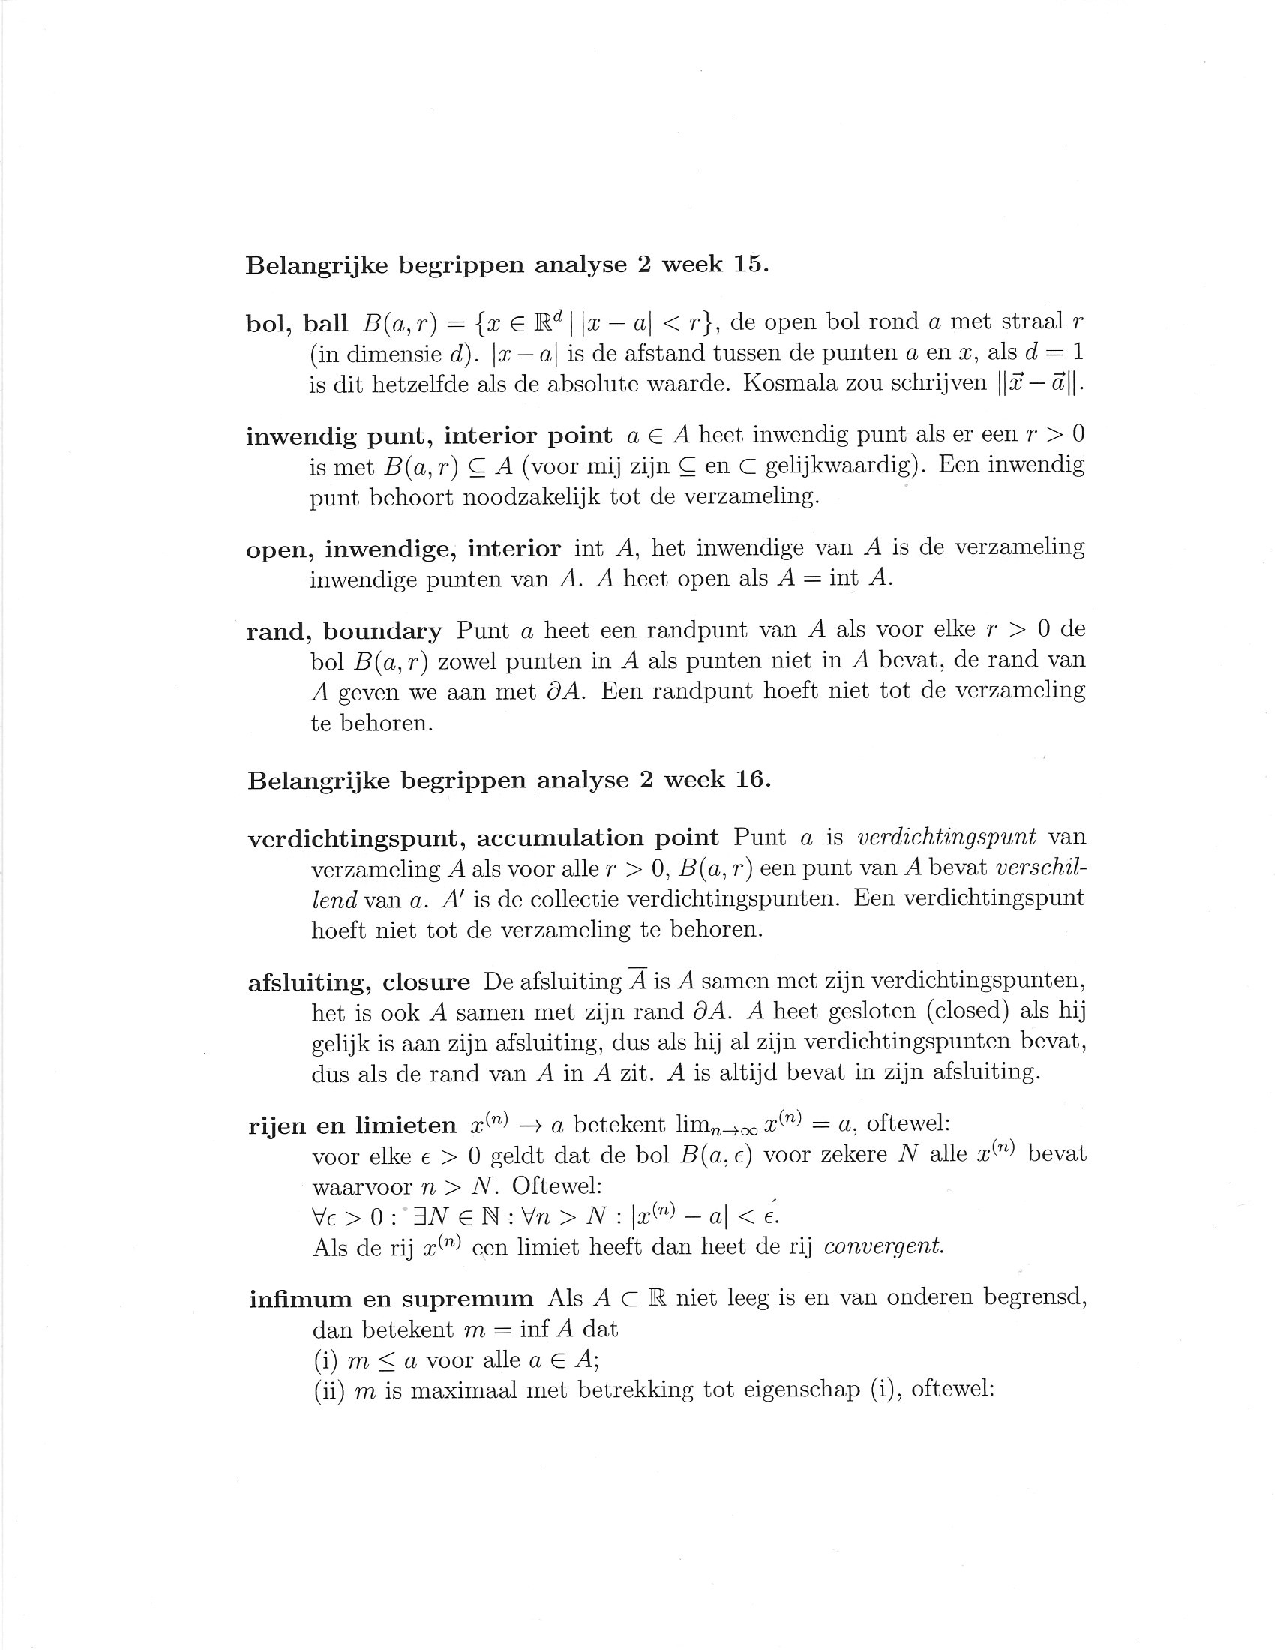
\includepdf[pages={-}]{Aart.pdf}
	
	\appendix
	\section{Appendix}
	
	\newpage
	\bibliographystyle{plain}
	\addcontentsline{toc}{chapter}{Bibliography}\bibliography{orgcite}
	\newpage
	\addcontentsline{toc}{chapter}{Index}
	\begin{scriptsize}\printindex\end{scriptsize}
\end{document}